\section{曲面的上同调环}
\sourcepage{356--357}
即使 $X$ 是 CW 复形，也没有计算其奇异上同调环的一般程序：胞腔链复形并不能确定环结构。两个空间可能有同构的胞腔链复形，却有不同构的上同调环。因此，我们转向单纯上同调，给出对应于奇异杯积的公式，再计算若干例子。

\entry{定义}{5.10.1}选取顶点偏序，使每个单形的顶点全序。定义单纯上链的杯积，使 $v_0<\cdots<v_{p+q}$ 时
\[
\langle c^p\smile c^q,[v_0,\ldots,v_{p+q}]\rangle
=\langle c^p,[v_0,\ldots,v_p]\rangle\langle c^q,[v_p,\ldots,v_{p+q}]\rangle.
\]
它与奇异公式十分相似。

\entry{定理}{5.10.2}给定排序后，单纯杯积双线性、结合，以每个顶点上取值 $1$ 的 $z^0$ 为单位，且满足上边缘公式
\[
\delta(c^p\smile c^q)=\delta c^p\smile c^q+(-1)^pc^p\smile\delta c^q.
\]
由该排序定义的链映射 $\eta$ 的对偶，将奇异杯积映为单纯杯积。

\textbf{证明：}各项直接验证；上边缘公式可重复定理 5.9.5 的计算，只改记号。另一证明是：$\eta$ 单射且将基元映为基元，像为直和项，所以其对偶满射。将给定单纯上链延拓为奇异上链，利用奇异公式，再用对偶保持杯积及上边缘，即得单纯公式。\hfill$\square$

\entry{定理}{5.10.3}单纯杯积诱导双线性、结合的上同调运算，不依赖顶点排序，以 $\{z^0\}$ 为单位，并被连续映射诱导的同态保持。

\textbf{证明：}由上边缘公式如前得良定义性。$\eta^*$ 是保持杯积的奇异到单纯上同调同构，且不依赖排序，所以单纯杯积也不依赖排序。它与连续映射诱导的同态可交换，而奇异上同调中的自然性已证，故得结论。\hfill$\square$

\sourcepage{358}
但单纯映射 $f$ 的上链映射 $f^\#$ 未必在\emph{上链层次}保持杯积，因为 $f$ 未必保持顶点排序。若只在有向单纯理论内部工作，这会使自然性证明相当困难。

整数与一般系数配对的杯积，以及相对子复形的杯积，也都存在。相对版本反而更容易：若两个因子分别在 $A,B$ 上为零，其积在 $A\cup B$ 上为零，因为并复形的每个单形必须属于其中之一。此时两子空间本来就是可切除对，奇异版本也有定义。

\entry{定义}{5.10.4}若任意两个正维上同调类之积均为零，称上同调环\textbf{平凡}。这不表示所有乘法为零，因为零维单位元的作用始终存在。

\entry{例}{5.10.5}取环面 $T$ 及图 5.10.1 的上闭链 $w^1,z^1$。记 $\alpha=\{w^1\}$、$\beta=\{z^1\}$，它们生成 $H^1(T)$；任一逆时针二维单形的初等上链之类记为 $\Lambda$，生成 $H^2(T)$。
\begin{center}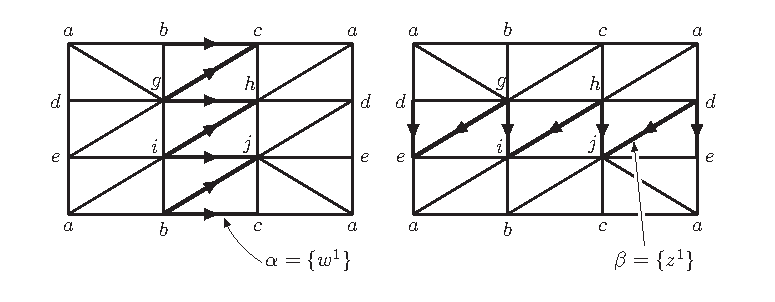
\includegraphics[width=.96\textwidth]{figures/5-10-1.pdf}\\图 5.10.1\end{center}
按字母顺序排列顶点。一个二维单形只有同时有面落在两个上链的载体中时，乘积才可能非零，因此只需考察 $[g,h,i]$、$[h,i,j]$。直接计算
\begin{align*}
\langle w^1\smile z^1,[g,h,i]\rangle&=1\cdot1=1,\\
\langle w^1\smile z^1,[h,i,j]\rangle&=(-1)\cdot0=0.
\end{align*}
故 $w^1\smile z^1=[g,h,i]^*$。这个单形顺时针定向，所以 $\alpha\smile\beta=-\Lambda$。

\sourcepage{359}
反向相乘时，两项分别为 $0\cdot(-1)=0$、$1\cdot1=1$，故 $z^1\smile w^1=[h,i,j]^*$，得到 $\beta\smile\alpha=\Lambda$，符合分次交换律。

直接计算还可得 $\alpha^2=\beta^2=0$。也可把 $w^1$ 换为与它上同调的图 5.10.2 中的 $y^1$，其载体与原栅栏分开，没有二维单形同时碰到两者，故 $w^1\smile y^1=0$。另一证明利用 $\alpha^2=-\alpha^2$，而 $H^2(T)$ 无二阶元素，所以平方为零。
\begin{center}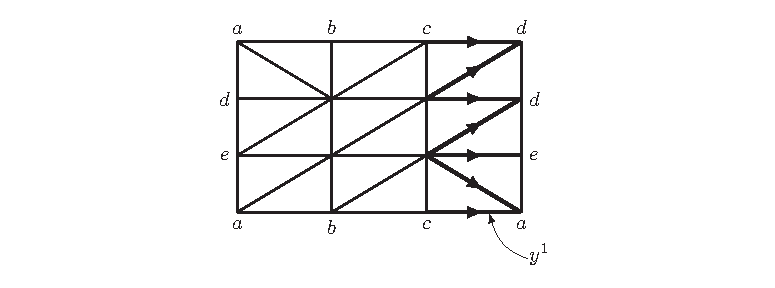
\includegraphics[width=.96\textwidth]{figures/5-10-2.pdf}\\图 5.10.2\end{center}
省略单位元，乘法表为
\[
\begin{array}{c|ccc}
\smile&\alpha&\beta&\Lambda\\\hline
\alpha&0&-\Lambda&0\\
\beta&\Lambda&0&0\\
\Lambda&0&0&0
\end{array}
\]
最后一行、一列因维数原因均为零。

\sourcepage{360}
\entry{例}{5.10.6}计算 Klein 瓶 $S$ 的模二上同调环。仍用 $\alpha=\{w^1\}$、$\beta=\{z^1\}$、$\Lambda=\{\sigma^*\}$，代表如图 5.10.3。上例的部分计算模二后仍成立：$\alpha\beta=\Lambda$，$\alpha^2=0$，后者可借助图 5.10.4 中的 $y^1$。
\begin{center}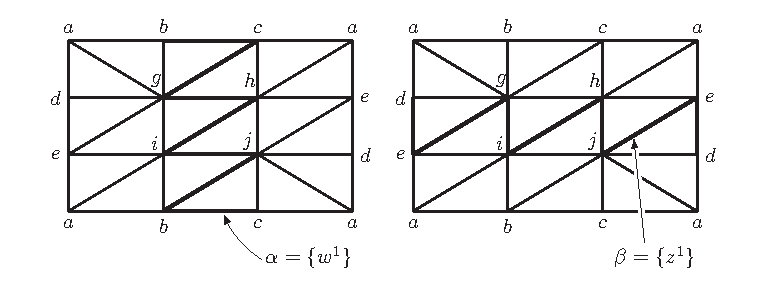
\includegraphics[width=.96\textwidth]{figures/5-10-3.pdf}\\图 5.10.3\end{center}
但 $z^1$ 不能像前者那样从自身移开，必须直接计算其平方。它在 $[d,e,g]$、$[e,g,i]$、$[d,e,j]$ 上取 $1$，其余为零，所以其类为 $3\Lambda=\Lambda$，即 $\beta^2=\Lambda$。

\sourcepage{361}
\begin{center}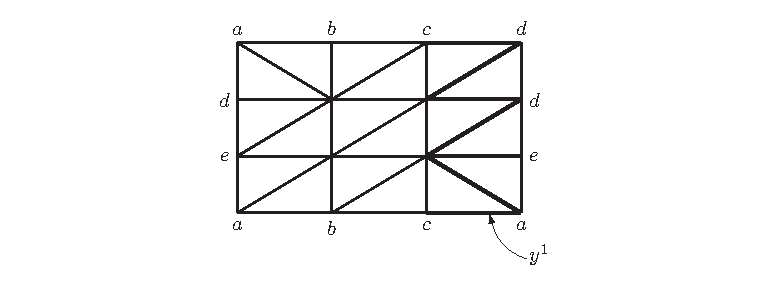
\includegraphics[width=.96\textwidth]{figures/5-10-4.pdf}\\图 5.10.4\end{center}
于是乘法表为
\[
\begin{array}{c|ccc}
\smile&\alpha&\beta&\Lambda\\\hline
\alpha&0&\Lambda&0\\
\beta&\Lambda&\Lambda&0\\
\Lambda&0&0&0
\end{array}
\]

\entry{例}{5.10.7}再计算 $P^2\#P^2$ 的模二上同调环。图 5.10.5 给出一个零维胞腔、两个一维胞腔及一个二维胞腔。取一维基本闭链
\[
w_1=[a,b]+[b,c]+[c,a],\qquad z_1=[a,d]+[d,e]+[e,a],
\]
二维基本链 $\gamma$ 为所有逆时针二维单形之和。它们满足 $\partial w_1=\partial z_1=0$、$\partial\gamma=-2w_1-2z_1$，故模二对偶的所有上边缘为零。因此 $H^1\cong(\Z/2)^2$、$H^2\cong\Z/2$。

图中的 $w^1,z^1$ 在上述两个基本闭链上的取值构成单位矩阵，所以其类 $\epsilon,\zeta$ 为一维上同调基。记二维生成元为 $\Lambda$。

\sourcepage{362}
\begin{center}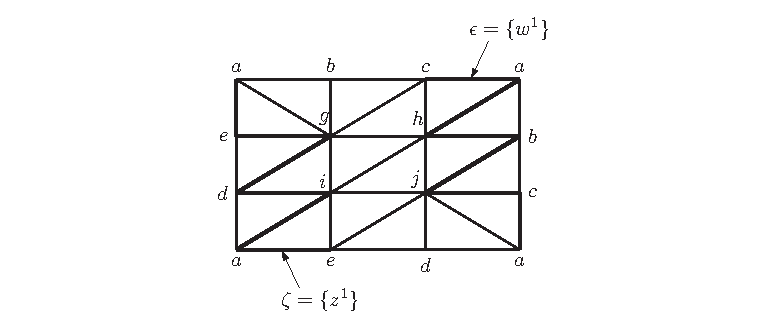
\includegraphics[width=.96\textwidth]{figures/5-10-5.pdf}\\图 5.10.5\end{center}
直接计算得到 $w^1\smile z^1=0$、$w^1\smile w^1=[a,c,j]^*$、$z^1\smile z^1=[a,e,g]^*$。因此
\[
\begin{array}{c|ccc}
\smile&\epsilon&\zeta&\Lambda\\\hline
\epsilon&\Lambda&0&0\\
\zeta&0&\Lambda&0\\
\Lambda&0&0&0
\end{array}
\]
然而 $P^2\#P^2$ 同胚于 Klein 瓶，所以这个环与上一例同构，虽然乘法表看起来很不一样。构造同构留给读者。这说明仅看不同基下的乘法表，通常不能立刻判断两个环是否同构。

\entry{例}{5.10.8}取图 5.10.6 的 $X=S^1\vee S^1\vee S^2$，即两个圆周与一个球面共用一点的\textbf{楔和}（wedge product）。它同样有零维一个、二维一个、一维两个胞腔，基本链为
\[
w_1=[a,b]+[b,c]+[c,a],\quad z_1=[a,d]+[d,e]+[e,a],\quad z_2=\partial[a,f,g,h].
\]
所有胞腔边缘为零，所以它与环面具有同构的胞腔链复形、同调群和上同调群。

\sourcepage{363}
\begin{center}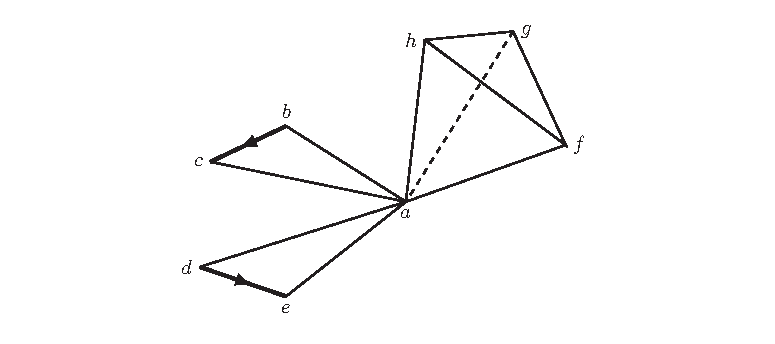
\includegraphics[width=.96\textwidth]{figures/5-10-6.pdf}\\图 5.10.6\end{center}
但上同调环不同。上闭链 $w^1=[b,c]^*$、$z^1=[d,e]^*$ 限制后为胞腔上链群的一组对偶基；没有二维单形具有其载体中的边，所以这些生成元之间的杯积全为零，环平凡。而环面的环不平凡。

这些例子说明杯积通常不易计算，困难在于必须进入单纯层次，找到具体上闭链代表。任何提供一般杯积信息的定理都很有价值。以后将证明两个这样的定理：一个描述乘积空间的上同调环，另一个描述流形的上同调环，特别能用于计算射影空间。

\sourcepage{364--365}
\subsection*{习题}
以下 $T$ 表示环面，$S$ 表示 Klein 瓶。
\begin{enumerate}
\item 若 $f:S^2\to T$ 连续，证明 $f^*:H^2(T)\to H^2(S^2)$ 为零，从而 $f_*:H_2(S^2)\to H_2(T)$ 为零。对 $g:T\to S^2$ 能说什么？
\item 证明下列情形中 $f^*:H^2(Y;\Z/2)\to H^2(X;\Z/2)$ 为零：$X=S^2,Y=S$；$X=S,Y=T$；$X=T,Y=S$。
\item 写出下列环的乘法表：$n$ 重环面连通和的整数上同调环；$P^2$ 的模二上同调环；$n$ 重实射影平面连通和的模二上同调环。
\item 构造例 5.10.6 与例 5.10.7 两个环之间的同构。\translatornote{原书此题引为例 5.10.5 与 5.10.6，但这两例的系数及群均不同，不可能同构；按前文留作习题的说明，应指后两例。}
\item 比较 Klein 瓶与 $P^2\vee S^1$。
\begin{enumerate}[label=(\alph*)]
\item 证明整数上同调环同构。
\item 证明模二上同调环不同构。注意仅给出不同乘法表还不足以证明。
\end{enumerate}
\item 计算三重愚人帽的模三上同调环。
\item \begin{enumerate}[label=(\alph*)]
\item 对 Möbius 带及其边界 $(M,E)$，计算模二相对与绝对上同调之间的杯积，以及两个相对因子之间的杯积。
\item 对圆柱面 $M=S^1\times I$、$E=S^1\times\Bd I$ 重复 (a)。
\end{enumerate}
\begin{center}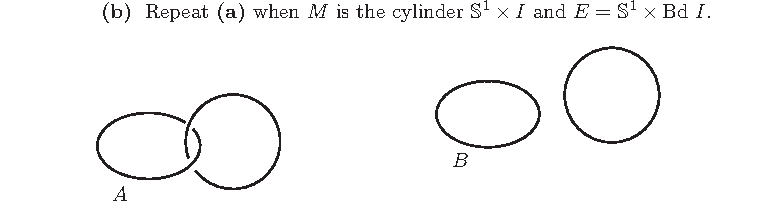
\includegraphics[width=.96\textwidth]{figures/5-10-7.pdf}\\图 5.10.7\end{center}
\item 设 $A$ 为 $S^3$ 中两个一次套链的圆周之并，$B$ 为两个不套链的圆周之并，见图 5.10.7。证明它们补空间的上同调群同构，但上同调环不同构。
\item 对上一题的同调能说什么？
\end{enumerate}
